
%% ============================================================
%%  CHƯƠNG 4: THỰC NGHIỆM VÀ ĐÁNH GIÁ
%% ============================================================
\chapter{Thực nghiệm và đánh giá}

\section{Môi trường thực nghiệm}
\label{sec:exp_setup}

Tất cả các đánh giá được thực hiện bằng Python 3, sử dụng framework Torch phiên bản 2.12.0, CUDA 13.2 cùng với các thư viện khác như Scikit-learn, NumPy, Pandas, pickle... Các thực nghiệm được tiến hành trên một máy Windows Subsystems for Linux (WSL2) với cấu hình CPU Intel Core \textsuperscript{\textregistered} i9-13900K (16 nhân 2.9 GHz), RAM 22 GB và ổ cứng 1TB SSD NVMe Gen 4.

\subsection{Tiền xử lý dữ liệu}
Bộ dữ liệu được sử dụng trong nghiên cứu này là CICIoT2023 \cite{ciciot2023}, một tập dữ liệu phát hiện xâm nhập quy mô lớn được thu thập trên hạ tầng thiết bị IoT thực tế. Trước khi đưa vào huấn luyện, dữ liệu thô được làm sạch bằng cách loại bỏ các bản ghi mang giá trị rỗng, giá trị vô cực hoặc bản ghi trùng lặp, đồng thời các đặc trưng số được chuẩn hoá về cùng một thang đo để tránh việc một vài đặc trưng có biên độ lớn lấn át quá trình học. Sau bước chuẩn hoá, mỗi luồng mạng được biểu diễn bằng một vector đặc trưng $20$ chiều, trong đó $20$ cột đầu đóng vai trò là đầu vào của mô hình còn cột cuối cùng lưu nhãn lớp tương ứng.

Tập đặc trưng $20$ chiều bao quát nhiều khía cạnh của một luồng mạng, từ đặc tính thsời gian, kích thước và thống kê gói, đến các cờ giao thức TCP cùng tỉ lệ phân bố giao thức. Bảng \ref{tab:cic23_features} liệt kê đầy đủ $20$ đặc trưng, được nhóm lại theo bản chất nhằm thuận tiện cho phần thảo luận sau này. Việc giới hạn ở $20$ đặc trưng giúp giảm chi phí huấn luyện trong mô phỏng nhiều client, đồng thời vẫn bảo toàn các tín hiệu quan trọng để phân biệt lưu lượng bình thường với các nhóm tấn công.

\begin{table}[H]
\centering
\caption{Tập $20$ đặc trưng đầu vào của CICIoT2023.}
\label{tab:cic23_features}
\begin{tabular}{lp{0.62\linewidth}}
\hline
Nhóm đặc trưng & Tên đặc trưng \\
\hline
Thời gian luồng       & flow\_duration, IAT \\
Kích thước gói        & Tot size, Tot sum, AVG, Min, Max, Magnitue, Header\_Length \\
Cờ TCP (xuất hiện)    & syn\_flag\_number, ack\_flag\_number, psh\_flag\_number, rst\_flag\_number, fin\_flag\_number \\
Số đếm cờ TCP         & syn\_count, ack\_count, rst\_count \\
Tỉ lệ giao thức       & TCP, UDP, ICMP \\
\hline
\end{tabular}
\end{table}

Tập dữ liệu sau tiền xử lý chứa $46{,}905{,}384$ bản ghi trải trên $34$ lớp, gồm một lớp lưu lượng bình thường (BenignTraffic) và $33$ lớp tấn công thuộc nhiều nhóm khác nhau. Một đặc điểm nổi bật của CICIoT2023 là phân phối lớp mất cân bằng nghiêm trọng: lớp đa số DDoS-ICMP\_Flood chiếm $15.42\%$ tổng số bản ghi, trong khi lớp Uploading\_Attack chỉ có $1{,}257$ mẫu. Sự chênh lệch hàng nghìn lần giữa lớp giàu nhất và lớp nghèo nhất khiến cho việc phát hiện các lớp thiểu số trở thành thách thức trọng tâm, đặc biệt khi dữ liệu lại tiếp tục bị phân mảnh và lệch nhãn trong môi trường học liên kết.

\subsection{Phân bổ dữ liệu phi IID}
Toàn bộ tập dữ liệu sau tiền xử lý được phân hoạch cho client theo ngữ cảnh Non-IID, đồng thời một tập kiểm thử toàn cục được giữ cố định và dùng chung cho mọi thuật toán nhằm bảo đảm việc so sánh diễn ra trên cùng một thước đo. Tập kiểm thử này được tách theo phân tầng giữ nguyên tỉ lệ lớp, nên phân phối nhãn trên tập kiểm thử trùng khớp với phân phối trên toàn tập, qua đó các lớp thiểu số vẫn hiện diện đầy đủ trong quá trình đánh giá.

Sau khi dữ liệu được tách theo lớp, mỗi lớp được phân bổ cho client theo ngữ cảnh Non-IID lệch nhãn (label skew), trong đó số mẫu của một lớp trên các client được lấy từ phân phối Dirichlet:
\[
\pi_c\sim \operatorname{Dir}(\alpha\mathbf{1}_{|K|}),
\qquad
n_{k,c}=\left\lfloor \pi_{k,c}N_c\right\rfloor,
\]
trong đó $N_c$ là số mẫu của lớp $c$, $|K|$ là số client và $n_{k,c}$ là số mẫu lớp $c$ được cấp cho client $k$. Vì phép lấy mẫu được lặp lại độc lập cho từng lớp, một client có thể giàu dữ liệu ở vài lớp nhưng thiếu nghiêm trọng ở các lớp khác, phản ánh tình huống IDS trong đó mỗi tổ chức chỉ quan sát được một phần của không gian tấn công. Tham số $\alpha$ điều khiển mức độ lệch nhãn; trong các thí nghiệm chính, $\alpha=0.1$ được sử dụng để tái tạo ngữ cảnh lệch nhãn nghiêm trọng.

\begin{figure*}[ht]
\centering
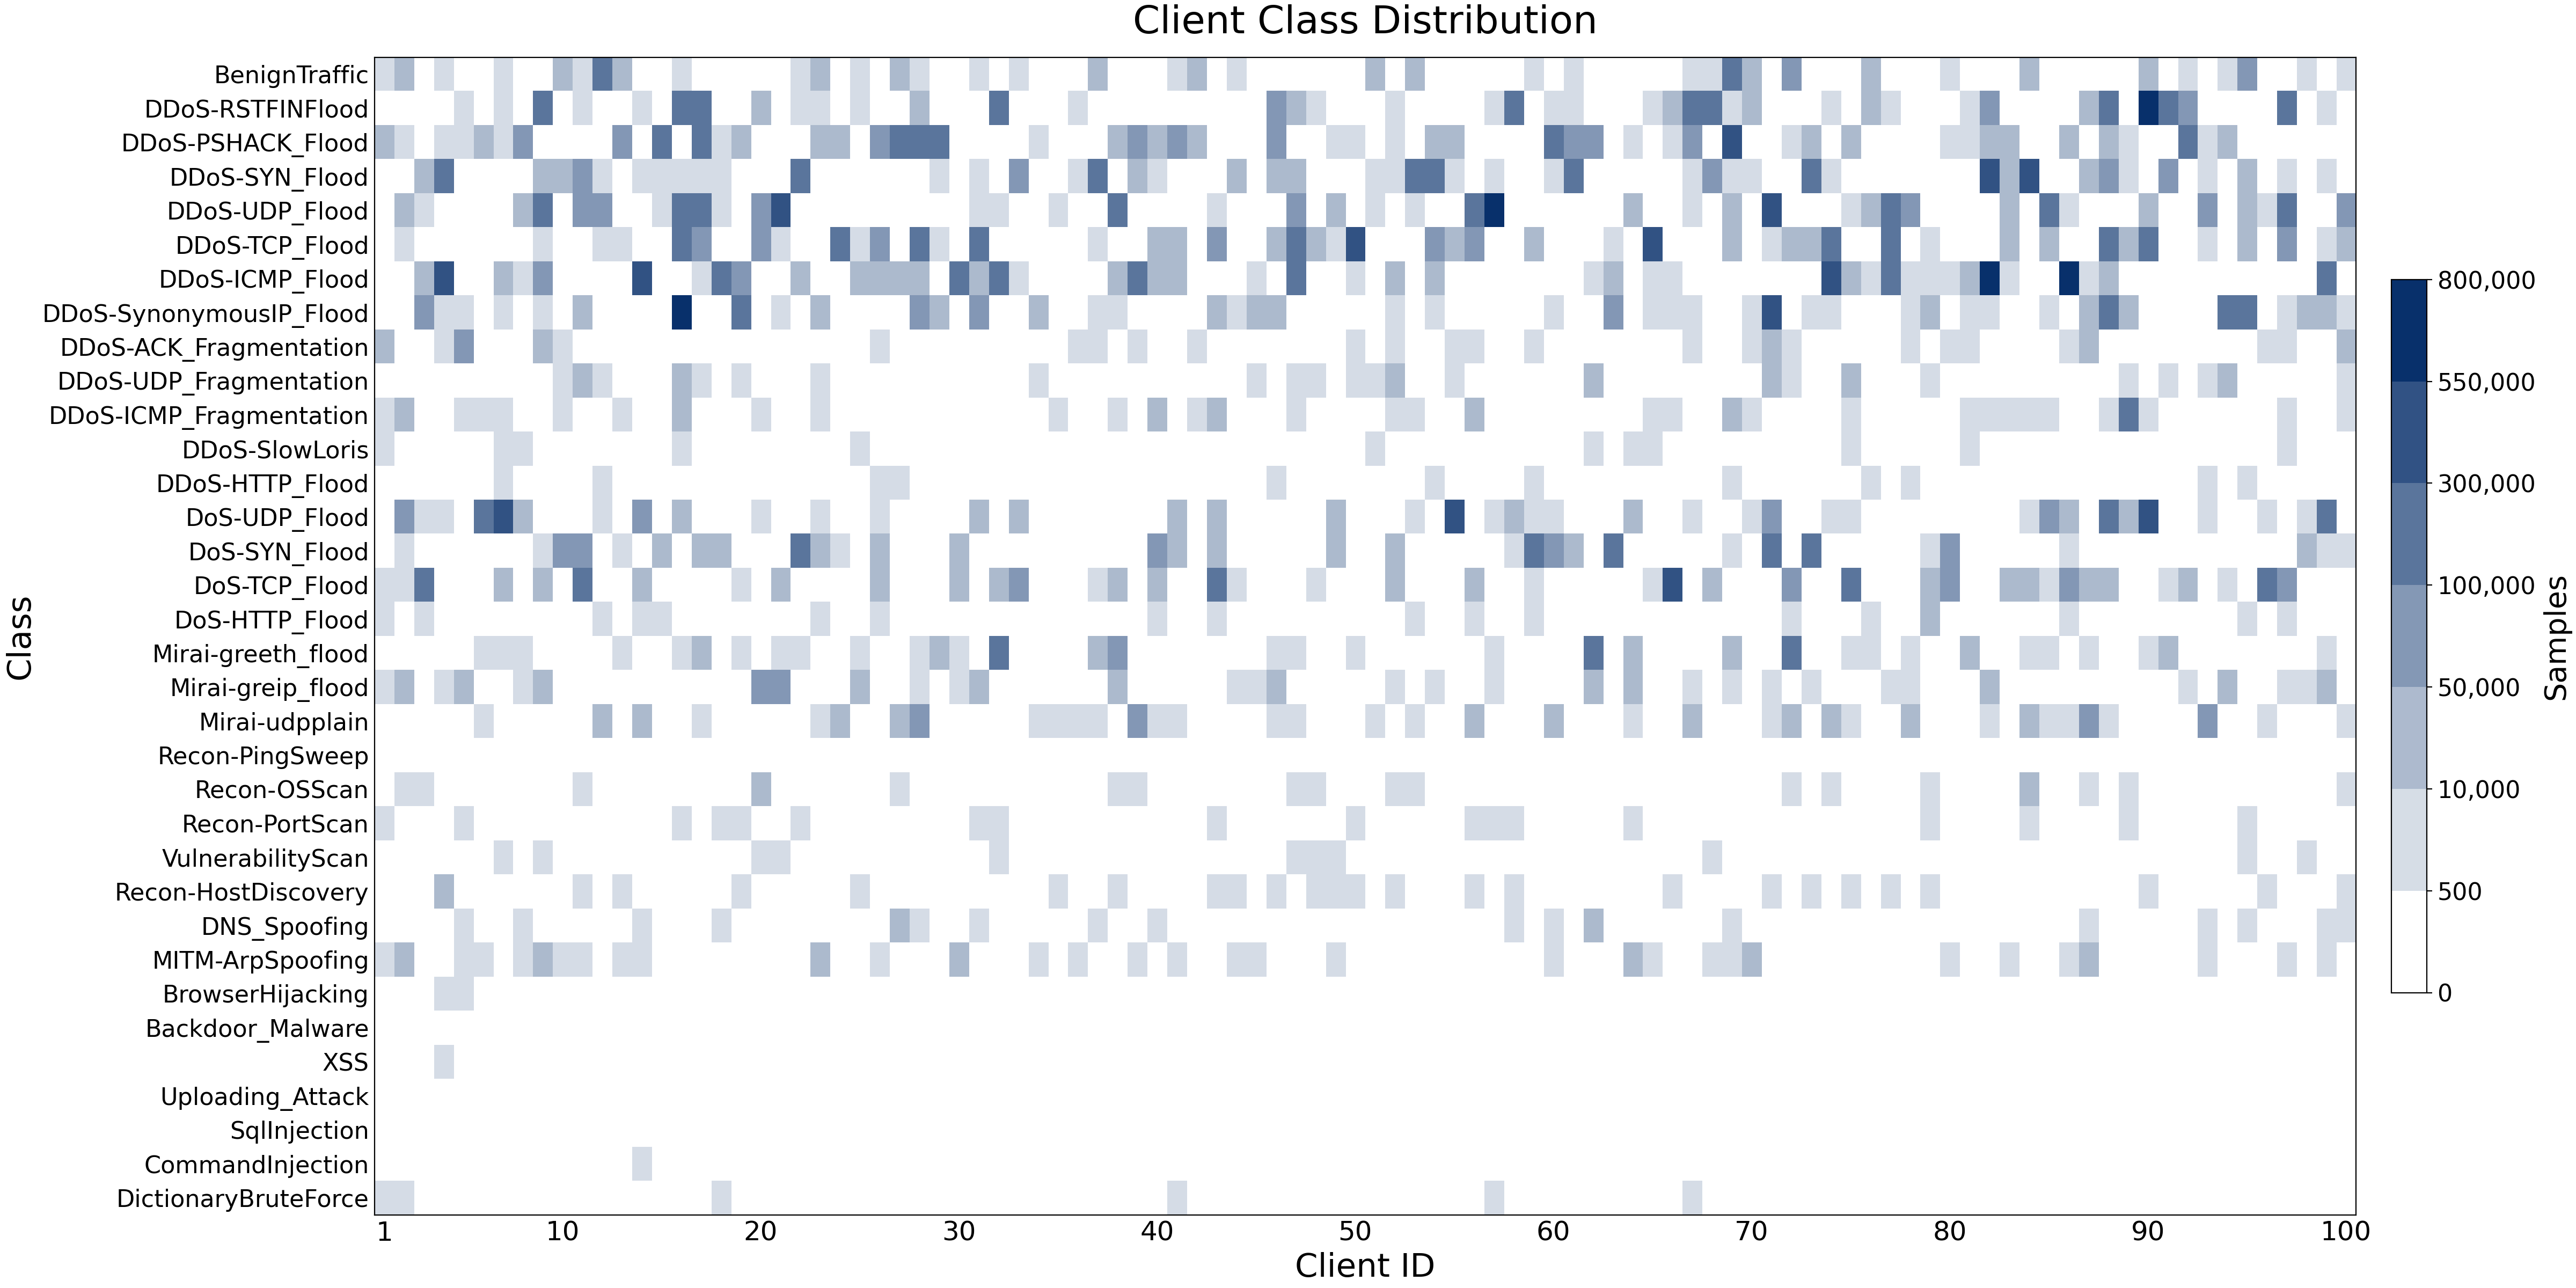
\includegraphics[width=1.0\textwidth]{images/partition.png}
\caption{Phân phối dữ liệu theo lớp cho 100 client.}
\label{fig:partition}
\end{figure*}

Sau khi phân hoạch, một tỉ lệ ngẫu nhiên trong khoảng $[5\%, 20\%]$ số mẫu của từng client được tách ra làm phần dữ liệu công khai, phần còn lại giữ làm dữ liệu riêng. Vì tỉ lệ cắt được lấy độc lập cho mỗi client, tổng phần công khai trên toàn hệ thống là $7{,}935{,}448$ mẫu ($16.92\%$), còn $38{,}969{,}936$ mẫu ($83.08\%$) được giữ làm dữ liệu riêng cho huấn luyện giám sát cục bộ.

\section{Các chỉ số đánh giá}
\label{sec:metrics}

Hiệu quả của giải pháp đề xuất được đánh giá bằng các chỉ số tiêu chuẩn sau:

\paragraph{Accuracy (Acc)} Chỉ số này là tỷ lệ các mẫu được dự đoán đúng trên tổng số mẫu trong tập kiểm tra:

\begin{equation}
\label{eq:accuracy}
\text{Acc} = \frac{TP + TN}{\text{Tổng số mẫu}}
\end{equation}

\paragraph{Precision} Tỷ lệ các mẫu dương tính được dự đoán đúng trên tất cả các mẫu được dự đoán là dương tính:

\begin{equation}
\label{eq:precision}
\text{Precision} = \frac{TP}{TP + FP}
\end{equation}

\paragraph{Recall} Tỷ lệ các mẫu dương tính được dự đoán đúng trên tất cả các mẫu dương tính thực tế:

\begin{equation}
\label{eq:recall}
\text{Recall} = \frac{TP}{TP + FN}
\end{equation}

\paragraph{F1-Score} Trung bình điều hòa của Precision và Recall:

\begin{equation}
\label{eq:f1}
\text{F1} = 2 \cdot \frac{\text{Precision} \cdot \text{Recall}}{\text{Precision} + \text{Recall}}
\end{equation}

trong đó $TP$ là số mẫu dương tính được dự đoán đúng, $TN$ là số mẫu âm tính được dự đoán đúng, $FP$ là số mẫu âm tính bị dự đoán sai thành dương tính, và $FN$ là số mẫu dương tính bị dự đoán sai thành âm tính.

Trong các bảng kết quả thực nghiệm, Precision, Recall và F1-Score được tính theo trung bình macro (macro-averaging), tức là tính toán các chỉ số trên từng lớp riêng biệt rồi lấy trung bình cộng. Phương pháp này phù hợp với dữ liệu mạng vốn mất cân bằng lớp nghiêm trọng, tránh trường hợp các lớp đa số lấn át các lớp thiểu số.

\section{Kịch bản thực nghiệm}
\label{sec:scenarios}
Để đánh giá toàn diện hiệu quả của DFD-IDS, các kịch bản thực nghiệm sau được xây dựng:

\subsection{Kịch bản không tấn công}
Trong kịch bản này, tất cả clients đều trung thực, không có tác nhân Byzantine. Mục tiêu là đánh giá hiệu suất cơ bản của DFD-IDS trong môi trường lý tưởng và so sánh với các phương pháp FL truyền thống.

\subsection{Kịch bản tấn công data poisoning}
Ở kịch bản data poisoning, một tỉ lệ client sẽ đóng vai Byzantine, mỗi client Byzantine sử dụng kỹ thuật Targetted Label Flipping \cite{tolpegin2020targetedflip} để lật nhãn của lớp có nhiều dữ liệu trong tập dữ liệu cục bộ của nó nhất thành nhãn Benign.

\subsection{Kịch bản tấn công đầu độc trọng số mô hình}
Ở kịch bản đầu độc trọng số mô hình, một tỉ lệ client sử dụng kỹ thuật PoisonedFL \cite{xie2025poisonedfl} để thống nhất cùng gửi một cập nhật đầu độc có khả năng thích nghi qua từng vòng liên kết.

PoisonedFL là một phương pháp tấn công Byzantine không toàn tri (non-omniscient) nhắm vào các phòng thủ FL. Điểm mới chính của PoisonedFL là hướng tấn công nhất quán và cường độ được tính toán qua nhiều vòng. Các client Byzantine thỏa thuận một ma trận dấu chung $s \in \{-1, +1\}^d$ và tạo ra một bản cập nhật mô hình đầu độc $g^t_b = s \odot k^t$, trong đó $k^t = \lambda^t \cdot v^t$ với $\lambda^t$ kiểm soát cường độ và $v^t$ kiểm soát hướng của vector tấn công. Vector $v^t$ được tính dựa trên chênh lệch giữa bản cập nhật tổng hợp và bản cập nhật đầu độc đã chuẩn hóa từ vòng trước, nhằm căn chỉnh cường độ tấn công với cường độ của các bản cập nhật lành tính. Hệ số $\lambda^t$ được điều chỉnh thích ứng dựa trên giả thuyết $H_0$ (tấn công không hiệu quả) hoặc $H_1$ (tấn công thành công), sử dụng phép kiểm định nhị thức trên số chiều của mô hình toàn cục. Nếu $H_0$ được chấp nhận, cường độ tấn công bị giảm theo hệ số $\beta < 1$ để tránh bị phát hiện. PoisonedFL tận dụng tính không đồng nhất tự nhiên của dữ liệu Non-IID để che giấu các cập nhật độc hại, khiến nó trở thành một trong những cuộc tấn công nguy hiểm nhất trong bối cảnh FL.

PoisonedFL là kỹ thuật tấn công Byzantine dành cho các thuật toán FL có tồn tại một mô hình toàn cục. Vì các thuật toán FD không sử dụng mô hình toàn cục, PoisonedFL đã được thiết kế lại để thích nghi với FD. Cụ thể, để ước tính mô hình toàn cục cho PoisonedFL, mỗi client Byzantine thực hiện học chắt lọc trên bộ consensus hoặc tập biểu diễn trung gian.

\begin{itemize}
    \item Ở các thuật toán sử dụng dữ liệu công khai, các client PoisonedFL chỉ cần chắt lọc hoặc học giám sát trên tập dữ liệu công khai này.
    \item Trong các thậut toán không sử dụng dữ liệu công khai như FedProto, các client PoisonedFL kết hợp dữ liệu của chính nó và chắt lọc trên biểu diễn toàn cục (global prototypes) để ước tính mô hình toàn cục, sau đó chúng trung bình cộng các bản mô hình đã được ước tính thành một mô hình toàn cục sau cùng để tính toán cập nhật bị đầu độc.
\end{itemize}

Do điều kiện không toàn tri, các client PoisonedFL chỉ có thể bắt đầu tấn công khi đã có ít nhất hai bộ biểu diễn trung gian, hai bộ mô hình toàn cục, hoặc hai bộ consensus.

Mỗi kịch bản tấn công được đánh giá với các tỷ lệ Byzantine khác nhau (20\%, 50\%) để quan sát biểu hiện của các phương pháp so sánh ở điều kiện tỉ lệ Byzantine bình thường và tỉ lệ Byzantine chiếm gần đa số.

\subsection{Kịch bản đa kiến trúc mô hình}
Trong kịch bản này, tập client được chia ra $4$ nhóm mô hình, trong đó nhóm $1$ sử dụng mô hình GRU, nhóm $2$ sử dụng mô hình DCNN-BiLSTM, nhóm $3$ sử dụng mô hình MLP và nhóm cuối cùng sử dụng mô hình CNN.


\section{Thiết lập mô hình}
\label{sec:model_setup}

Các mô hình chính trong thí nghiệm được hiện thực bằng PyTorch. Đầu vào của mỗi mô hình là vector đặc trưng $x\in\mathbb{R}^{20}$, còn đầu ra là vector logits có kích thước bằng số lớp hiện tại. Trong chế độ dự đoán, logits được đưa qua hàm softmax để tạo phân phối xác suất; trong huấn luyện, loss được tính trực tiếp trên logits để giữ ổn định số học.

Tất cả các mô hình phân loại dùng Adam làm bộ tối ưu. Learning rate mặc định được co giãn theo batch size:
\[
\eta=10^{-3}\sqrt{\frac{B}{1024}},
\]
trong đó $B$ là batch size. Batch size mặc định là $8192$. Learning rate dùng warm-up tuyến tính:
\[
\eta_e=\eta\frac{e+1}{5}.
\]
Hàm mất mát cho học giám sát là cross-entropy với label smoothing $0.05$. Gradient được chuẩn hoá bằng clipping theo chuẩn $\ell_2$ với ngưỡng $0.5$. Một số lớp tuyến tính được áp dụng weight decay $10^{-4}$ để giảm overfitting, trong khi các tham số còn lại không dùng weight decay. Các mô hình dùng LayerNorm thay cho BatchNorm vì thí nghiệm có batch lớn, dữ liệu Non-IID và phân phối giữa client khác nhau; LayerNorm giúp chuẩn hoá biểu diễn theo từng mẫu và ít phụ thuộc thống kê batch hơn.

\subsection{Mô hình GRU}
\label{sec:gru_arch}

GRU \cite{kasongo2023gru} xử lý vector 20 chiều như chuỗi một chiều có độ dài 20, mỗi bước thời gian chứa một giá trị đặc trưng. Cách biểu diễn này cho phép mô hình học quan hệ tuần tự tương đối giữa các đặc trưng sau tiền xử lý, đồng thời vẫn giữ chi phí thấp hơn BiLSTM. Bảng \ref{tab:gru_arch} trình bày kiến trúc GRU.

\begin{table}[H]
\centering
\caption{Kiến trúc GRU dùng trong thí nghiệm.}
\label{tab:gru_arch}
\begin{tabularx}{\textwidth}{l c X}
\hline
Tầng & Kích thước & Thiết lập \\
\hline
Reshape & $20\rightarrow20\times1$ & Mỗi đặc trưng là một bước chuỗi \\
GRU 1 & $1\rightarrow128$ & Trả về toàn bộ chuỗi, LayerNorm, Dropout $0.15$ \\
GRU 2 & $128\rightarrow128$ & Trả về toàn bộ chuỗi, LayerNorm, Dropout $0.15$ \\
GRU 3 & $128\rightarrow128$ & Lấy trạng thái cuối, LayerNorm, Dropout $0.15$ \\
Dense head & $128\rightarrow64$ & ReLU, LayerNorm, Dropout $0.20$ \\
Classifier & $64\rightarrow C$ & Logits theo số lớp $C$ \\
\hline
\end{tabularx}
\end{table}

Ba tầng GRU liên tiếp cho phép mô hình tích luỹ tương tác phi tuyến giữa các đặc trưng. Hai tầng đầu giữ toàn bộ chuỗi để tầng sau tiếp tục xử lý thông tin theo vị trí đặc trưng, còn tầng cuối chỉ lấy trạng thái cuối làm biểu diễn toàn cục. Dense head dùng ReLU vì đây là tầng nén cuối trước logits, cần ánh xạ rõ ràng và gọn hơn thay vì giữ dạng kích hoạt trơn như MLP.

\subsection{Mô hình DCNN--BiLSTM}
\label{sec:dcblstm_arch}

DCNN--BiLSTM \cite{hnamte2023dcnnbilstm} là mô hình sâu hơn, kết hợp trích xuất mẫu cục bộ bằng tích chập một chiều và mô hình hoá phụ thuộc hai chiều bằng BiLSTM. Bảng \ref{tab:dcblstm_arch} mô tả kiến trúc của mô hình này.

\begin{table}[H]
\centering
\caption{Kiến trúc CNN--BiLSTM dùng trong thí nghiệm.}
\label{tab:dcblstm_arch}

\begin{tabularx}{\textwidth}{l c X}
\hline
Tầng & Kích thước & Thiết lập \\
\hline
Reshape & $20\rightarrow1\times20$ & Một kênh đầu vào \\
Conv1D & $1\rightarrow64$ & Kernel size $20$, padding same, ReLU, LayerNorm \\
BiLSTM 1 & $64\rightarrow2\times64$ & Trả về toàn bộ chuỗi, LayerNorm \\
BiLSTM 2 & $128\rightarrow2\times128$ & Lấy trạng thái cuối hai chiều, Dropout $0.10$ \\
DNN 1 & $256\rightarrow64$ & ReLU, Dropout $0.10$ \\
DNN 2 & $64\rightarrow32$ & ReLU, Dropout $0.10$ \\
DNN 3 & $32\rightarrow16$ & ReLU, Dropout $0.10$ \\
LayerNorm & $16$ & Chuẩn hoá biểu diễn cuối \\
Classifier & $16\rightarrow C$ & Logits theo số lớp $C$ \\
\hline
\end{tabularx}
\end{table}

Tầng CNN đầu tiên đóng vai trò bộ trích xuất mẫu cục bộ trên toàn bộ vector đặc trưng. Do kernel size bằng số chiều đầu vào, mỗi filter học một phép chiếu có cấu trúc qua toàn bộ đặc trưng, sau đó BiLSTM khai thác biểu diễn theo hai hướng. Việc dùng hai tầng BiLSTM giúp mô hình học cả quan hệ thấp và quan hệ trừu tượng hơn, còn khối DNN cuối giảm chiều biểu diễn trước khi phân loại.

\subsection{Mô hình Multi Layer Perceptron}

MLP được dùng làm mô hình đơn giản cho dữ liệu vector 20 chiều. Kiến trúc này ưu tiên độ ổn định và tốc độ, phù hợp với các thí nghiệm nhiều client. Bảng \ref{tab:mlp_arch} mô tả các tầng chính.

\begin{table}[H]
\centering
\caption{Kiến trúc MLP dùng trong thí nghiệm.}
\label{tab:mlp_arch}
\begin{tabular}{lll}
\hline
Tầng & Kích thước & Thiết lập \\
\hline
Input & $20$ & Vector đặc trưng luồng mạng \\
LayerNorm & $20$ & Chuẩn hoá đầu vào \\
Linear 1 & $20\rightarrow128$ & SiLU, LayerNorm, Dropout $0.15$ \\
Linear 2 & $128\rightarrow128$ & SiLU, LayerNorm, Dropout $0.20$, residual \\
Linear 3 & $128\rightarrow64$ & SiLU, LayerNorm, Dropout $0.15$ \\
Classifier & $64\rightarrow C$ & Logits theo số lớp $C$ \\
\hline
\end{tabular}
\end{table}

Hàm kích hoạt SiLU được chọn thay cho ReLU ở các tầng ẩn vì SiLU có dạng trơn, giảm hiện tượng gradient bằng không ở vùng âm và thường ổn định hơn trên dữ liệu bảng sau chuẩn hoá. Kết nối residual ở tầng $128\rightarrow128$ giúp mô hình học hiệu chỉnh trên biểu diễn trung gian thay vì phải tái tạo toàn bộ ánh xạ.

\subsection{Mô hình CNN}

CNN một chiều là một mô hình có kiến trúc nông, đóng vai trò straggler trong kịch bản mô hình hỗn hợp, nơi một phần client chạy kiến trúc nông và nhẹ hơn so với GRU hay DCNN--BiLSTM. Vector đặc trưng $20$ chiều được xem như một chuỗi một kênh, sau đó được xử lý qua ba khối tích chập một chiều liên tiếp nhằm trích xuất mẫu cục bộ ở nhiều mức độ trừu tượng. Bảng \ref{tab:cnn_arch} mô tả các tầng chính của kiến trúc này.

\begin{table}[H]
\centering
\caption{Kiến trúc CNN dùng làm mô hình straggler.}
\label{tab:cnn_arch}
\begin{tabular}{lll}
\hline
Tầng & Kích thước & Thiết lập \\
\hline
Reshape & $20\rightarrow1\times20$ & Một kênh đầu vào \\
Conv1D 1 & $1\rightarrow32$ & Kernel $3$, padding $1$, BatchNorm, ReLU, Dropout $0.15$ \\
MaxPool 1 & $/2$ & Giảm chiều theo hệ số $2$ \\
Conv1D 2 & $32\rightarrow64$ & Kernel $3$, padding $1$, BatchNorm, ReLU, Dropout $0.15$ \\
MaxPool 2 & $/2$ & Giảm chiều theo hệ số $2$ \\
Conv1D 3 & $64\rightarrow64$ & Kernel $3$, padding $1$, BatchNorm, ReLU, Dropout $0.15$ \\
GAP & $64$ & Adaptive average pooling \\
FC & $64\rightarrow64$ & SiLU, LayerNorm, Dropout $0.20$ \\
Classifier & $64\rightarrow C$ & Logits theo số lớp $C$ \\
\hline
\end{tabular}
\end{table}

Khác với các kiến trúc còn lại vốn dựa trên LayerNorm, các khối tích chập của CNN được chuẩn hoá bằng BatchNorm, do biểu diễn tích chập ổn định hơn khi được chuẩn hoá theo từng kênh trên toàn batch. Sau ba khối tích chập, một tầng adaptive average pooling nén chuỗi đặc trưng về một vector cố định, nhờ đó phần đầu phân loại không phụ thuộc vào độ dài chuỗi trung gian.

\section{Kết quả thực nghiệm}
\label{sec:results}

\newcommand{\topone}[1]{\cellcolor{green!90!black}#1}
\newcommand{\toptwo}[1]{\cellcolor{green!60!black}#1}
\newcommand{\topthree}[1]{\cellcolor{green!30}#1}

\subsection{Kết quả thực nghiệm trong môi trường không tấn công}
Trong môi trường lành tính (không có client Byzantine), DFD-IDS đạt hiệu suất cạnh tranh so với các phương pháp Học liên kết tập trung, đồng thời mang lại các lợi ích bổ sung như điều phối phân tán và chi phí truyền thông giảm. Cơ chế Energy-based Vote Abstention lọc hiệu quả các dự đoán không chắc chắn, tạo ra một consensus sạch hơn cho quá trình chắt lọc kiến thức.

\begin{table}[H]
\centering
\small
\caption{Kịch bản không tấn công}
\label{tab:benign}
\begin{tabularx}{\textwidth}{lccccX}
\toprule
\textbf{Phương pháp} & \textbf{Acc} & \textbf{Recall (macro)} & \textbf{Precision (macro)} & \textbf{F1 (macro)} \\
\midrule
\multicolumn{6}{c}{\textbf{Federated Distillation (FD)}} \\
\midrule
Đề xuất           & 0.9415 & \toptwo{0.5401} & 0.5121 & 0.5056 \\
SSFL-IDS & \toptwo{0.9605} & \topone{0.5831} & \toptwo{0.5849} & \topone{0.5651}\\
FedKD-IDS  & 0.9484 & 0.5015 & 0.4894 & 0.4795 \\
FedProto  & 0.3968 & 0.2072 & 0.108 & 0.1223 \\
\midrule
\multicolumn{6}{c}{\textbf{Federated Learning (FL)}} \\
\midrule
FedAvg & \topone{0.9656} & 0.5141 & \topone{0.5851} & \topthree{0.5105} \\
FLAME  & 0.9454 & \topthree{0.5368} & \topthree{0.5520} & \toptwo{0.5112} \\
\bottomrule
\end{tabularx}
\end{table}

\begin{table}[H]
\centering
\small
\caption{Kịch bản không tấn công -- đa kiến trúc mô hình}
\label{tab:mixed_benign}
\begin{tabularx}{\textwidth}{lccccX}
\toprule
\textbf{Phương pháp} & \textbf{Acc} & \textbf{Recall (macro)} & \textbf{Precision (macro)} & \textbf{F1 (macro)}\\
\midrule
Đề xuất           & \topone{0.9346} & \toptwo{0.471} & \toptwo{0.4745} & \toptwo{0.4553} \\
SSFL-IDS          & \toptwo{0.8943} & \topone{0.4922} & \topone{0.4972} & \topone{0.4735} \\
FedKD-IDS         & \topthree{0.7785} & \topthree{0.467} & \topthree{0.43} & \topthree{0.4267} \\
FedProto          & 0.5400 & 0.321 & 0.2171 & 0.2273 \\
\bottomrule
\end{tabularx}
\end{table}

\subsection{Kết quả thực nghiệm trong môi trường Byzantine}
\subsubsection{Tấn công Targeted Flip}

\begin{table}[H]
\centering
\small
\caption{Kết quả tấn công Targeted Flip (tỉ lệ Byzantine 0.2)}
\label{tab:targeted_flip0.2}
\begin{tabularx}{\textwidth}{lccccX}
\toprule
\textbf{Phương pháp} & \textbf{Acc} & \textbf{Recall (macro)} & \textbf{Precision (macro)} & \textbf{F1 (macro)} \\
\midrule
\multicolumn{6}{c}{\textbf{Federated Distillation (FD)}} \\
\midrule
Đề xuất           & \toptwo{0.9582} & \topone{0.5500} & \topthree{0.5131} & \toptwo{0.5188}  \\
SSFL-IDS & \topthree{0.9550} & 0.5069 & 0.4981 & 0.4904 \\
FedKD-IDS & 0.9500 & 0.5138 & 0.5079 & 0.4928 \\
FedProto   & 0.5666 & 0.3355 & 0.2242 & 0.2399 \\
\midrule
\multicolumn{6}{c}{\textbf{Federated Learning (FL)}} \\
\midrule
FedAvg     & \topone{0.9674} & \topthree{0.5272} & \topone{0.6153} & \topthree{0.5182} \\
FLAME      & 0.9088 & \toptwo{0.5386} & \toptwo{0.5738} & \topone{0.5211}\\
\bottomrule
\end{tabularx}
\end{table}

\begin{table}[H]
\centering
\small
\caption{Đa kiến trúc mô hình dưới tấn công Targeted Flip (tỉ lệ Byzantine 0.2)}
\label{tab:mixed_targeted_flip0.2}
\begin{tabularx}{\textwidth}{lccccX}
\toprule
\textbf{Phương pháp} & \textbf{Acc} & \textbf{Recall (macro)} & \textbf{Precision (macro)} & \textbf{F1 (macro)}  \\
\midrule
Đề xuất           & \topone{0.9306} & \toptwo{0.4882} & \toptwo{0.487} & \toptwo{0.4713}\\
SSFL-IDS          & \toptwo{0.8954} & \topone{0.4897} & \topone{0.4976} & \topone{0.4763}\\
FedKD-IDS         & \topthree{0.7758} & \topthree{0.4487} & \topthree{0.4061} & \topthree{0.3992}\\
FedProto          & 0.5487 & 0.3263 & 0.2253 & 0.2335\\
\bottomrule
\end{tabularx}
\end{table}

\begin{table}[H]
\centering
\small
\caption{Kết quả tấn công Targeted Flip (tỉ lệ Byzantine 0.5)}
\label{tab:targeted_flip0.5}
\begin{tabularx}{\textwidth}{lccccX}
\toprule
\textbf{Phương pháp} & \textbf{Acc} & \textbf{Recall (macro)} & \textbf{Precision (macro)} & \textbf{F1 (macro)}  \\
\midrule
\multicolumn{6}{c}{\textbf{Federated Distillation (FD)}} \\
\midrule
Đề xuất           & \topthree{0.8431} & \topthree{0.476} & 0.4684 & \topthree{0.4427} \\
SSFL-IDS & \toptwo{0.9575} & \toptwo{0.5397} & \toptwo{0.5347} & \toptwo{0.5178}\\
FedKD-IDS & 0.7346 & 0.3974 & 0.3184 & 0.3383\\
FedProto   & 0.5565 & 0.3266 & 0.2165 & 0.2317\\
\midrule
\multicolumn{6}{c}{\textbf{Federated Learning (FL)}} \\
\midrule
FedAvg     & \topone{0.9726} & \topone{0.5449} & \topone{0.6119} & \topone{0.5357} \\
FLAME      & 0.6889 & 0.4746 & \topthree{0.4846} & 0.4246 \\
\bottomrule
\end{tabularx}
\end{table}

\begin{table}[H]
\centering
\small
\caption{Đa kiến trúc mô hình dưới tấn công Targeted Flip (tỉ lệ Byzantine 0.5)}
\label{tab:mixed_targeted_flip0.5}
\begin{tabularx}{\textwidth}{lccccX}
\toprule
\textbf{Phương pháp} & \textbf{Acc} & \textbf{Recall (macro)} & \textbf{Precision (macro)} & \textbf{F1 (macro)} \\
\midrule
Đề xuất           & \toptwo{0.9281} & \toptwo{0.4965} & \toptwo{0.4781} & \toptwo{0.4675} \\
SSFL-IDS          & \topone{0.951} & \topone{0.5057} & \topone{0.485} & \topone{0.4878} \\
FedKD-IDS         & \topthree{0.822} & \topthree{0.4598} & \topthree{0.427} & \topthree{0.4259} \\
FedProto          & 0.5263 & 0.3137 & 0.2055 & 0.2178 \\
\bottomrule
\end{tabularx}
\end{table}

\subsubsection{Tấn công PoisonedFL}

\begin{table}[H]
\centering
\small
\caption{Kết quả tấn công PoisonedFL (tỉ lệ Byzantine 0.2)}
\label{tab:poisonedfl0.2}
\begin{tabularx}{\textwidth}{lccccX}
\toprule
\textbf{Phương pháp} & \textbf{Acc} & \textbf{Recall (macro)} & \textbf{Precision (macro)} & \textbf{F1 (macro)} \\
\midrule
\multicolumn{6}{c}{\textbf{Federated Distillation (FD)}} \\
\midrule
Đề xuất           & \topone{0.9554} & \topone{0.5250} & \topone{0.5024} & \topone{0.5063} \\
SSFL-IDS          & 0.0061 & 0.0294 & 0.0002 & 0.0004 \\
FedKD-IDS         & \topthree{0.7173} & \topthree{0.3043} & \topthree{0.2583} & \topthree{0.2570} \\
FedProto          & 0.1508 & 0.0573 & 0.0168 & 0.0213 \\
\midrule
\multicolumn{6}{c}{\textbf{Federated Learning (FL)}} \\
\midrule
FedAvg            & 0.0235 & 0.0294 & 0.0007 & 0.0014\\
FLAME             & \toptwo{0.7292} & \toptwo{0.4237} & \toptwo{0.4576} & \toptwo{0.3808} \\
\bottomrule
\end{tabularx}
\end{table}

\begin{table}[H]
\centering
\small
\caption{Đa kiến trúc mô hình dưới tấn công PoisonedFL (tỉ lệ Byzantine 0.2)}
\label{tab:mixed_poisonedfl0.2}
\begin{tabularx}{\textwidth}{lccccX}
\toprule
\textbf{Phương pháp} & \textbf{Acc} & \textbf{Recall (macro)} & \textbf{Precision (macro)} & \textbf{F1 (macro)} \\
\midrule
Đề xuất           & \topone{0.918} & \topone{0.4739} & \topone{0.4636} & \topone{0.4505} \\
SSFL-IDS          & \topthree{0.0887} & \topthree{0.0341} & \topthree{0.0323} & \topthree{0.0323} \\
FedKD-IDS         & \toptwo{0.784} & \toptwo{0.4397} & \toptwo{0.4607} & \toptwo{0.4065} \\
FedProto          & 0.0235 & 0.0294 & 0.0007 & 0.0014 \\
\bottomrule
\end{tabularx}
\end{table}

\begin{table}[H]
\centering
\small
\caption{Kết quả tấn công PoisonedFL (tỉ lệ Byzantine 0.5)}
\label{tab:poisonedfl0.5}
\begin{tabularx}{\textwidth}{lccccX}
\toprule
\textbf{Phương pháp} & \textbf{Acc} & \textbf{Recall (macro)} & \textbf{Precision (macro)} & \textbf{F1 (macro)}\\
\midrule
\multicolumn{6}{c}{\textbf{Federated Distillation (FD)}} \\
\midrule
Đề xuất           & \toptwo{0.6951} & \toptwo{0.3595} & \toptwo{0.2833} & \toptwo{0.2798}\\
SSFL-IDS          & 0.0235 & 0.0294 & 0.0007 & 0.0014  \\
FedKD-IDS         & \topone{0.9572} & \topone{0.5396} & \topone{0.5276} & \topone{0.5188} \\
FedProto          & \topthree{0.1087} & \topthree{0.0411} & \topthree{0.0101} & \topthree{0.0125} \\
\midrule
\multicolumn{6}{c}{\textbf{Federated Learning (FL)}} \\
\midrule
FedAvg            & 0.0235 & 0.0294 & 0.0007 & 0.0014 \\
FLAME             & 0.0617 & 0.0239 & 0.0098 & 0.0092 \\
\bottomrule
\end{tabularx}
\end{table}

\begin{table}[H]
\centering
\small
\caption{Đa kiến trúc mô hình dưới tấn công PoisonedFL (tỉ lệ Byzantine 0.5)}
\label{tab:mixed_poisonedfl0.5}
\begin{tabularx}{\textwidth}{lccccX}
\toprule
\textbf{Phương pháp} & \textbf{Acc} & \textbf{Recall (macro)} & \textbf{Precision (macro)} & \textbf{F1 (macro)} \\
\midrule
FedKD-IDS         & \topone{0.8483} & \topone{0.3915} & \topone{0.4346} & \topone{0.3732} \\
Đề xuất           & \toptwo{0.4561} & \toptwo{0.2758} & \toptwo{0.1987} & \toptwo{0.1968} \\
SSFL-IDS          & \topthree{0.0235} & \topthree{0.0294} & \topthree{0.0007} & \topthree{0.0014} \\
FedProto          & \topthree{0.0235} & \topthree{0.0294} & \topthree{0.0007} & \topthree{0.0014} \\
\bottomrule
\end{tabularx}
\end{table}

\subsection{Phân tích kết quả}

Trong kịch bản không tấn công, Đề xuất đạt Accuracy $0.9415$ và F1 macro $0.5056$, thấp hơn SSFL-IDS và FedAvg ở một vài chỉ số tổng quát nhưng vẫn duy trì vùng hiệu năng cạnh tranh. Điểm đáng chú ý là loss của Đề xuất thấp thứ hai trong toàn bảng, cho thấy quá trình chắt lọc tạo ra dự đoán tương đối ổn định ngay cả khi hệ thống không có client độc hại. Điều này phù hợp với mục tiêu thiết kế: phương pháp không chỉ tối ưu một mô hình toàn cục duy nhất, mà tạo consensus từ các dự đoán đủ tin cậy để làm tín hiệu huấn luyện chung.

Ở tấn công Targeted Flip với tỉ lệ Byzantine $0.2$, Đề xuất đứng trong nhóm dẫn đầu trên Accuracy, Recall macro, F1 macro và đạt loss thấp nhất. Kết quả này cho thấy cơ chế lọc theo năng lượng và hợp nhất logits không chỉ loại bớt các dự đoán bất thường mà còn giữ lại đủ tín hiệu của các client lành tính để bảo toàn hiệu quả phân loại. Khi tỉ lệ Byzantine tăng lên $0.5$, hiệu năng của Đề xuất giảm rõ rệt, nhưng vẫn cao hơn FedKD-IDS, FedProto và FLAME ở Accuracy. Sự suy giảm này phản ánh giới hạn tự nhiên của đồng thuận khi số client độc hại tiến gần đa số; tuy nhiên phương pháp vẫn không sụp đổ hoàn toàn như một số cơ chế phòng thủ dựa vào khoảng cách hoặc prototype đơn giản.

Trong kịch bản PoisonedFL, sự khác biệt giữa các phương pháp trở nên rõ hơn. Với tỉ lệ Byzantine $0.2$, Đề xuất đạt kết quả tốt nhất trên toàn bộ các chỉ số chính và giữ loss thấp nhất, trong khi FedAvg và SSFL-IDS gần như mất khả năng phân loại. Điều này cho thấy việc không trực tiếp tổng hợp trọng số mô hình giúp Đề xuất tránh được hướng tấn công vốn được thiết kế để thao túng cập nhật tham số. Ở tỉ lệ Byzantine $0.5$, FedKD-IDS đạt kết quả cao nhất, còn Đề xuất giảm xuống mức trung gian. Dù vậy, Đề xuất vẫn vượt xa FedAvg, SSFL-IDS, FedProto và FLAME, cho thấy hệ thống còn giữ được một phần khả năng kháng nhiễu ngay cả khi tín hiệu độc hại chiếm tỉ trọng rất lớn.

Trong cấu hình đa kiến trúc mô hình (các bảng đánh dấu ``đa kiến trúc'' trong từng kịch bản), Đề xuất cho thấy ưu điểm hệ thống quan trọng. Trong môi trường không tấn công và Targeted Flip, phương pháp duy trì Accuracy trên $0.92$ và thường nằm trong nhóm hai phương pháp tốt nhất, dù các client sử dụng GRU, DCNN--BiLSTM, MLP và CNN đồng thời. Ở PoisonedFL với tỉ lệ Byzantine $0.2$, Đề xuất tiếp tục dẫn đầu tất cả các chỉ số chính, trong khi SSFL-IDS và FedProto gần như bị vô hiệu hoá. Khi tỉ lệ Byzantine tăng lên $0.5$, Đề xuất không còn đạt kết quả tốt nhất nhưng vẫn vượt SSFL-IDS và FedProto, cho thấy trao đổi logits trên dữ liệu công khai là một hướng phù hợp cho môi trường vừa bất đồng nhất kiến trúc vừa có nguy cơ Byzantine.

% \begin{table}[H]
% \centering
% \small
% \caption{So sánh độ chính xác của bộ lọc (Filter Accuracy) dưới tấn công PoisonedFL và Targeted Flip ở tỉ lệ 0.2}
% \label{tab:filter_accuracy0.2}
% \resizebox{\textwidth}{!}{%
% \begin{tabular}{lccccc}
% \toprule
% \textbf{Loại tấn công} & \textbf{Phương pháp} & \textbf{Accuracy} & \textbf{Precision} & \textbf{Recall} & \textbf{F1} \\
% \midrule
% \multirow{4}{*}{PoisonedFL (tỉ lệ 0.2)}
%  & Robust Logit Fusion  & 0.9300 & 0.7407 & 1.0000 & 0.8511 \\
%  & FedKD-IDS (Hamming) & 0.5200 & 0.2941 & 1.0000 & 0.4545 \\
% \midrule
% \multirow{3}{*}{PoisonedFL (đa kiến trúc, tỉ lệ 0.2)}
%  & Robust Logit Fusion & 0.8000 & 0.0000 & 0.0000 & 0.0000 \\
%  & FedKD-IDS (Hamming) & 0.3200 & 0.0000 & 0.0000 & 0.0000 \\
% \bottomrule
% \end{tabular}
% }
% \end{table}

% \begin{table}[H]
% \centering
% \small
% \caption{So sánh độ chính xác của bộ lọc (Filter Accuracy) dưới tấn công PoisonedFL và Targeted Flip ở tỉ lệ 0.5}
% \label{tab:filter_accuracy0.5}
% \resizebox{\textwidth}{!}{%
% \begin{tabular}{lccccc}
% \toprule
% \textbf{Loại tấn công} & \textbf{Phương pháp} & \textbf{Filter Acc} & \textbf{Filter Prec} & \textbf{Filter Rec} & \textbf{Filter F1} \\
% \midrule
% \multirow{4}{*}{PoisonedFL (tỉ lệ 0.2)}
%  & Robust Logit Fusion  & 0.5000 & 1.0000 & 0.5000 & 0.6667 \\
%  & FedKD-IDS (Hamming) & 0.2000 & 0.0000 & 0.0000 & 0.0000 \\
% \midrule
% \multirow{3}{*}{PoisonedFL (đa kiến trúc, tỉ lệ 0.2)}
%  & Robust Logit Fusion & 0.5800 & 1.0000 & 0.5435 & 0.7042 \\
%  & FedKD-IDS (Hamming) & 0.2400 & 0.0000 & 0.0000 & 0.0000 \\
% \bottomrule
% \end{tabular}
% }
% \end{table}

\subsection{Nhận xét}
Từ bảng so sánh, có thể thấy:

\begin{itemize}
    \item DFD-IDS duy trì hiệu quả cạnh tranh trong môi trường lành tính, đồng thời tránh phụ thuộc vào việc tổng hợp trực tiếp trọng số mô hình như các phương pháp FL truyền thống.
    \item Trong các kịch bản PoisonedFL, phương pháp đề xuất thể hiện ưu thế rõ nhất khi tỉ lệ Byzantine ở mức 0.2, đặc biệt ở cấu hình đa kiến trúc nơi nhiều phương pháp so sánh gần như mất khả năng phân loại.
    \item Khi tỉ lệ Byzantine tăng lên 0.5, hiệu năng của Đề xuất suy giảm nhưng vẫn giữ được kết quả cao hơn các phương pháp bị sụp đổ hoàn toàn, cho thấy cơ chế lọc logits còn giữ được tín hiệu học hữu ích trong điều kiện tấn công mạnh.
    \item Bảng độ chính xác bộ lọc cho thấy Robust Logit Fusion phát hiện client độc hại ổn định hơn FedKD-IDS Hamming, đặc biệt trong kịch bản PoisonedFL tiêu chuẩn.
\end{itemize}

\pagebreak
